%% 
%% Copyright 2007-2024 Elsevier Ltd
%% 
%% This file is part of the 'Elsarticle Bundle'.
%% ---------------------------------------------
%% 
%% It may be distributed under the conditions of the LaTeX Project Public
%% License, either version 1.3 of this license or (at your option) any
%% later version.  The latest version of this license is in
%%    http://www.latex-project.org/lppl.txt
%% and version 1.3 or later is part of all distributions of LaTeX
%% version 1999/12/01 or later.
%% 
%% The list of all files belonging to the 'Elsarticle Bundle' is
%% given in the file `manifest.txt'.
%% 
%% Template article for Elsevier's document class `elsarticle'
%% with numbered style bibliographic references
%% SP 2008/03/01
%% $Id: elsarticle-template-num.tex 249 2024-04-06 10:51:24Z rishi $
%%
\documentclass[preprint,review,12pt]{elsarticle}

%% Use the option review to obtain double line spacing
%% \documentclass[authoryear,preprint,review,12pt]{elsarticle}

%% Use the options 1p,twocolumn; 3p; 3p,twocolumn; 5p; or 5p,twocolumn
%% for a journal layout:
%% \documentclass[final,1p,times]{elsarticle}
%% \documentclass[final,1p,times,twocolumn]{elsarticle}
%% \documentclass[final,3p,times]{elsarticle}
%% \documentclass[final,3p,times,twocolumn]{elsarticle}
%% \documentclass[final,5p,times]{elsarticle}
%% \documentclass[final,5p,times,twocolumn]{elsarticle}

%% For including figures, graphicx.sty has been loaded in
%% elsarticle.cls. If you prefer to use the old commands
%% please give \usepackage{epsfig}

%% The amssymb package provides various useful mathematical symbols
\usepackage{amssymb}
%% The amsmath package provides various useful equation environments.
\usepackage{multirow}
\usepackage{amsmath}
%% The amsthm package provides extended theorem environments
%% \usepackage{amsthm}
\usepackage{libertine}  % Libertine font, good readability
\usepackage{newtxmath}  % Math support for Libertine

%% The lineno packages adds line numbers. Start line numbering with
%% \begin{linenumbers}, end it with \end{linenumbers}. Or switch it on
%% for the whole article with \linenumbers.
%% \usepackage{lineno}

\journal{Expert Systems With Applications}

\begin{document}

\begin{frontmatter}

%% Title, authors and addresses

%% use the tnoteref command within \title for footnotes;
%% use the tnotetext command for theassociated footnote;
%% use the fnref command within \author or \affiliation for footnotes;
%% use the fntext command for theassociated footnote;
%% use the corref command within \author for corresponding author footnotes;
%% use the cortext command for theassociated footnote;
%% use the ead command for the email address,
%% and the form \ead[url] for the home page:
%% \title{Title\tnoteref{label1}}
%% \tnotetext[label1]{}
%% \author{Name\corref{cor1}\fnref{label2}}
%% \ead{email address}
%% \ead[url]{home page}
%% \fntext[label2]{}
%% \cortext[cor1]{}
%% \affiliation{organization={},
%%             addressline={},
%%             city={},
%%             postcode={},
%%             state={},
%%             country={}}
%% \fntext[label3]{}

\title{Enhancing Q-Learning for Intraday Financial Trading: Dynamic State Modeling with Attention LSTM and Physics-Informed Neural Networks}

%% use optional labels to link authors explicitly to addresses:
 \author[label1]{Muktinath Vishwakarma}
 \author[label2]{Jagdish Chakole}
 \author[label1]{Manish Kurhekar}

 \affiliation[label1]{organization={Visvesvaraya National Institute of Technology},
	%% addressline={},
	city={Nagpur},
	postcode={440010},
	state={Maharashtra},
	country={India}}
	
	 \affiliation[label2]{organization={Indian Institute of Information Technology},
		%% addressline={},
		city={Nagpur},
		postcode={441108},
		state={Maharashtra},
		country={India}}
	
%% Abstract
\begin{abstract}
 Data-driven trading is particularly well-suited for short-term trading, as stock prices are influenced by numerous factors, many of which are unknown or unpredictable. When the time window for trading is large, the likelihood of price movements being affected by external factors increases, making predictions less reliable. Intraday trading, on the other hand, relies heavily on recent trading activity and is inherently data-driven. Given that stock price data exhibits both temporal and spatial characteristics, effective trading strategies must account for these dynamics while addressing the market's ever-changing nature.
 
 In this research, we propose a novel Reinforcement Learning (RL) framework for intraday trading, where the RL agent refines its trading strategy through interactions with the stock market environment. A critical aspect of RL is the representation of the state space, as it directly impacts the agent's learning efficiency and decision-making capabilities. To this end, we introduce a unique method for state-space representation that leverages Long Short-Term Memory (LSTM) networks, Deep Neural Networks (DNN), and k-Means clustering.
 
 The LSTM component captures long-term temporal dependencies in the time-series data, while the DNN extracts spatial features, capturing complex patterns and relationships within the data. The k-Means clustering algorithm is then employed to discretize and combine these features into a finite, manageable state space for Q-learning. By integrating these components, our approach effectively models the intricate dynamics of the stock market, enabling the RL agent to make informed trading decisions.
 
 Our methodology is specifically tailored to the dynamic and high-frequency nature of intraday trading and represents a significant advancement in applying RL to financial markets. This novel state-space representation bridges the gap between the complexity of stock market data and the computational demands of traditional Q-learning methods, paving the way for more effective and efficient data-driven trading strategies.
\end{abstract}

%%Graphical abstract
%%\begin{graphicalabstract}
%\includegraphics{grabs}
%%\end{graphicalabstract}

%%Research highlights
%%\begin{highlights}
%%\item Research highlight 1
%%\item Research highlight 2
%%\end{highlights}

%% Keywords
\begin{keyword}
	Reinforcement Learning\sep LSTM\sep Deep Learning\sep Intraday Trading
%% keywords here, in the form: keyword \sep keyword

%% PACS codes here, in the form: \PACS code \sep code

%% MSC codes here, in the form: \MSC code \sep code
%% or \MSC[2008] code \sep code (2000 is the default)

\end{keyword}

\end{frontmatter}

%% Add \usepackage{lineno} before \begin{document} and uncomment 
%% following line to enable line numbers
%% \linenumbers

%% main text
%%

%% Use \section commands to start a section
\section{Introduction}

\subsection{Background and Motivation}
\subsection{Problem Statement}
\subsection{Objectives of the Research}
\subsection{Contributions and Novelty}
\section{Literature Review}
\subsection{Transformers in Financial Forecasting}
\subsection{Reinforcement Learning for Trading}
\subsection{ State Space Representation and Discretization in RL}
\subsection{Related Work on Combining Historical and Predictive Data}
\section{ Proposed System}
\subsection{Overview of the Proposed System}
	\begin{figure}[h]
		\centering
		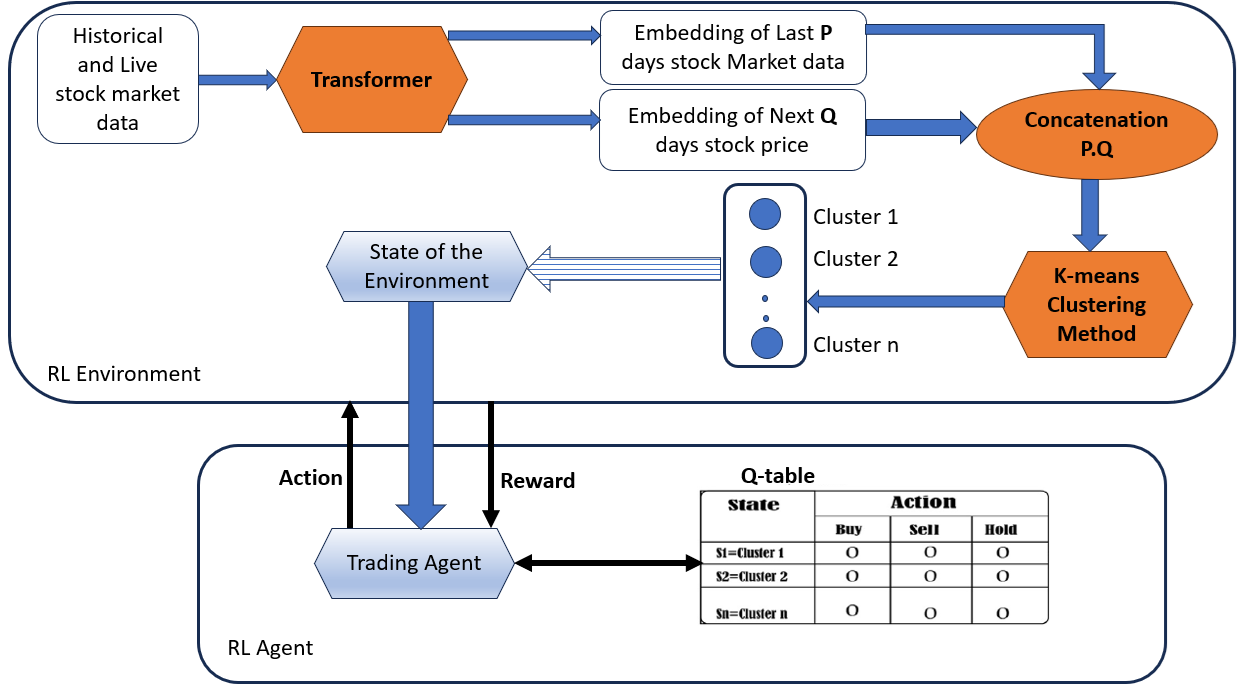
\includegraphics[width=0.9\textwidth, height=0.6\textheight]{Pmodel.png}
		\caption{Proposed model of the trading strategy.}
		\label{fig1l}
	\end{figure}

\subsection{ Transformer-Based State Encoding}
\subsection{Future Price Prediction Model}
\subsection{Discretization Techniques}
\subsection{Integration with Reinforcement Learning}
\section{Experimental Setup}
\subsection{Data Collection}
\subsection{Model Implementation}
\subsection{Evaluation Metrics}
\section{Results and Discussion}
\subsection{Performance Analysis}
\subsection{Comparison with Traditional Methods}
\subsection{Discussion of Findings}
\subsection{Conclusion and Future Work}
\section{Results and Discussion}
\subsection{Summary of Contributions}
\subsection{Implications for Financial Trading}
\subsection{Future Research Directions}

\bibliographystyle{elsarticle-num}
\bibliography{sample}
\end{document}
\endinput
%%
%% End of file `elsarticle-template-num.tex'.
